% !TEX root = ../../main.tex
\section{Forward Problem: Proof 2F}
\label{sec:forward-problem-proof2f}

We again start from the forward-problem assumption: a centripetal inverse-square law $a_F\propto 1/r^2$.
By Section~\ref{sec:forward-problem-hodograph}, this implies a circular hodograph in velocity space.
This section presents a second route, using that hodograph-circle nature directly through rotated/scaled auxiliary circles.
As in earlier sections, we intentionally over-scribe assisting lines so readers can spot more angle and length relations at a glance.
For each conic, a simpler base shape is enough for a minimal proof, but the enriched diagram exposes multiple valid relation chains.
In the subsections below we highlight several such chains so readers can develop alternative proof techniques from the same geometric idea.
Throughout this section, whenever the scale factors \(b^2/L\) (ellipse/hyperbola) or \(a^2/L\) (parabola, with \(a:=MF\)) appear, see \Cref{subsec:proof2f-discussion} for their equivalent expressions purely in initial data \((\mu,L,r_0,d_0)\). In the same notation, \(b^2/p=a\) and \(a^2/p=p/4\), so these geometric ratios are also determined by initial conditions.

\subsection{Ellipse: Forward Problem Proof 2F}
\label{subsec:ellipse-proof2f}

\begin{figure}[t]
  \centering
  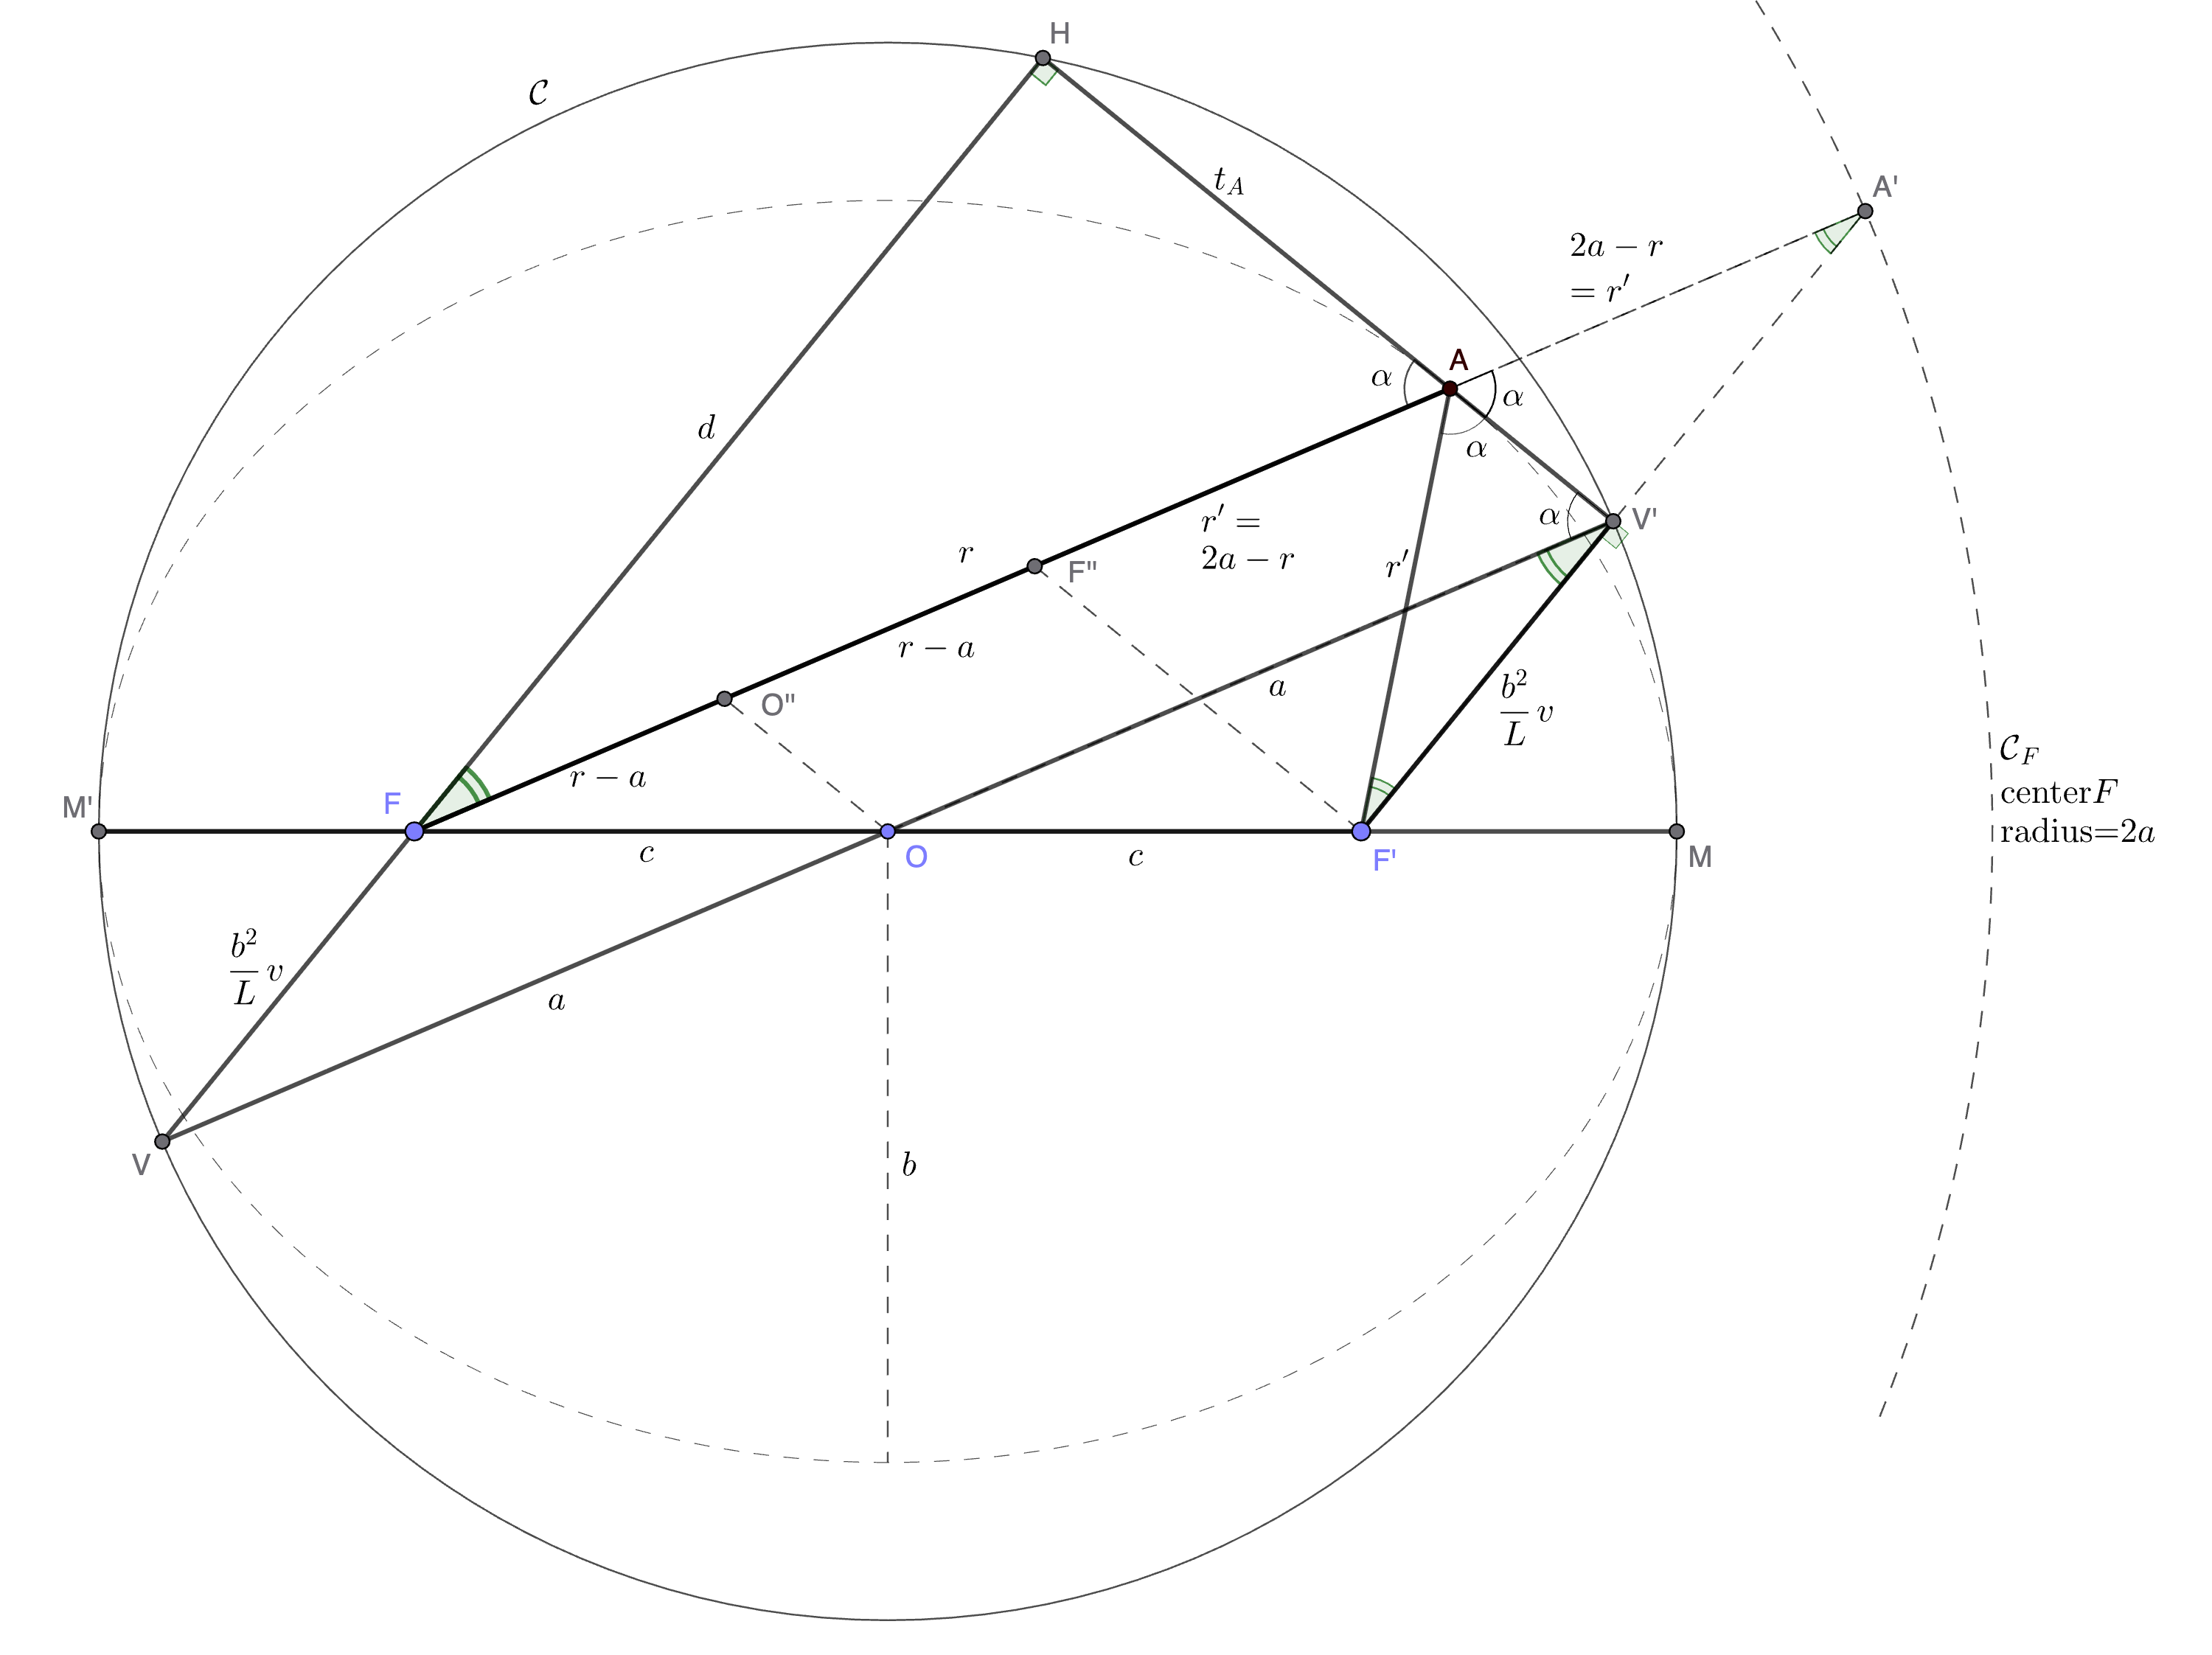
\includegraphics[width=\linewidth]{assets/images/ellipse_proof2F.png}
  \caption{Ellipse configuration for Forward Problem Proof~2F.}
  \label{fig:ellipse-proof2f}
\end{figure}

Using \Cref{fig:ellipse-proof2f}, we set up the elliptic Forward Problem Proof~2F in the circle-to-orbit framework.
In this subsection we also use the standard elliptic identity for the semi-latus rectum \(p\): geometrically, \(p\) is the perpendicular distance from the force center \(F\) to the orbit along the line through \(F\) orthogonal to the major axis. In \((a,b,c)\) notation,
\begin{equation}
  p^2+(2c)^2=(2a-p)^2
  \quad\Longrightarrow\quad
  p=\frac{a^2-c^2}{a}=\frac{b^2}{a}.
\label{eq:p-b2-over-a-ellipse}
\end{equation}

\begin{proposition}[Forward Problem Proof~2F: ellipse case]
Assume inverse-square centripetal attraction, so the hodograph is a circle. If the velocity origin lies inside that hodograph circle, then the orbit is an ellipse.
\end{proposition}

\begin{proof}
Start with the hodograph circle of radius $u$. Rotate it counterclockwise by $90^\circ$ and scale by $b^2/L$, where \(b\) is a length parameter left undetermined at this stage, and \(L\) is the specific angular momentum (twice areal speed, fixed by central-force motion from Section~2; later \(a,b,c\) are expressed from initial data in \Cref{eq:proof2f-disc-shodo-u-E0,eq:proof2f-disc-abc-from-initial}). Denote the scaled circle by $\mathcal C$ with center $O$, radius $a$, and
\[
  OF=:c,
  \qquad
  a=\frac{b^2}{L}u.
\]
Let the line $OF$ meet $\mathcal C$ at $M'$ (near $F$) and $M$ (far from $F$). For any point $V\in\mathcal C$, let the line $VF$ meet $\mathcal C$ again at $H$.

By the Euclidean power-of-a-point theorem (secant-secant form),
\[
  FM'\cdot FM = FV\cdot FH = (a-c)(a+c)=a^2-c^2.
\]
Write $FH=:d$ and, from the chosen scaling, $FV=\frac{b^2}{L}v$; then
\[
  a^2-c^2=\frac{b^2}{L}\,v\,d.
\]
Choose the scale parameter so that
\[
  b^2=a^2-c^2.
\]
Hence $v\,d=L$. Therefore, the point where the true velocity line (perpendicular to $FH$) meets the tangent line $t_A$ is exactly the constructed point $H$.

Now draw $t_A$ through $H$ perpendicular to $FH$, and let $V'$ be the second intersection of $t_A$ with $\mathcal C$. Since $\angle VHV'=90^\circ$, $VV'$ is a diameter of $\mathcal C$, so $O\in VV'$. Draw through $V'$ the line perpendicular to $HV'$ and let it meet $OF$ at $F'$. Then $F'V'\parallel VH$, and the corresponding triangles give
\[
  F'V'=FV=\frac{b^2}{L}v,
  \qquad
  OF'=OF=c.
\]
So $F'$ is uniquely determined as the reflection of $F$ across $O$, independent of the choice of $V$.

To locate the orbital point $A$ on $t_A$, use direction information: $OV$ is normal to $\mathcal C$ at $V$, hence normal to the local tangent proxy, so it is parallel to the acceleration direction. Because the force is centripetal, this gives
\[
  AF\parallel V'V.
\]
Let $A'=FA\cap F'V'$. Since $AF\parallel V'V$ and $O\in V'V$, we have $OV'\parallel FA'$. In $\triangle FF'A'$, $O$ is the midpoint of $FF'$ and $OV'\parallel FA'$, so $V'$ is the midpoint of $F'A'$. Therefore
\[
  FA'=2\,OV'=2a.
\]
Also, $A,V'\in t_A$, while $A'F'$ is collinear with $F'V'$ and $F'V'\perp t_A$; hence $AV'\perp A'F'$. Since $V'$ is the midpoint of $A'F'$, the line $AV'$ is the perpendicular bisector of $A'F'$. Therefore
\[
  AA'=AF',
  \qquad
  \angle V'AF'=\angle V'AA'.
\]
This is the reflection characterization at $A$ across the tangent line $t_A$. Combining $AA'=AF'$ with the distance relation above gives
\[
  AF+AF' = AF+AA' = FA' = 2a.
\]
This is the gardener characterization of an ellipse (constant sum of distances to two fixed foci), with foci $F,F'$. Therefore, when the velocity origin is inside the hodograph circle, the orbit is elliptic.
\end{proof}

\paragraph{Alternative closing step without constructing \(A'\): ellipse proof 2F'.}
\begin{proof}[Alternative proof (ellipse 2F')]
One may branch from the step \(AF\parallel V'V\) (just before introducing \(A'\)). Define
\[
  r:=FA,
  \qquad
  r':=F'A.
\]
Draw \(F'F''\parallel t_A\) and let it meet \(FA\) at \(F''\). Draw \(OO''\parallel t_A\) and let it meet \(FA\) at \(O''\) (on the branch from \(F\) to \(A\)).

Since \(O\in V'V\), the relation \(AF\parallel V'V\) implies \(AF\parallel OV'\). Also \(OO''\parallel t_A\parallel AV'\). Hence \(O''AV'O\) is a parallelogram, so
\[
  O''A=OV'=a,
\]
where \(OV'=a\) is the radius definition of \(\mathcal C\). Therefore
\[
  FO''=FA-O''A=r-a.
\]
In \(\triangle FF'F''\), \(O\) is the midpoint of \(FF'\), and \(OO''\parallel F'F''\); hence \(O''\) is the midpoint of \(FF''\), so
\[
  FF''=2\,FO''=2(r-a).
\]
Thus
\[
  AF''=AF-FF''=r-2(r-a)=2a-r.
\]

The reflection-angle relation at \(A\) used above can then be established via the right-triangle similarity \(\triangle AHF\sim\triangle AV'F'\), since \(V'F':FH=VF:FH=AV':AH\). Set
\[
  \angle FAH=\angle F'AV'=: \alpha.
\]
Because \(F'F''\parallel t_A\) and \(AV'\subset t_A\),
\[
  \angle AF''F'=\angle FAH=\alpha,
  \qquad
  \angle AF'F''=\angle F'AV'=\alpha.
\]
Hence \(\triangle AF'F''\) is isosceles, so \(AF''=AF'=r'\). Combining with \(AF''=2a-r\), we get
\[
  r'=2a-r
  \quad\Longrightarrow\quad
  r+r'=2a.
\]
This is exactly the gardener characterization of an ellipse, completing the same conclusion without constructing \(A'\), i.e., the alternative ellipse Proof~2F'.
\end{proof}

At this stage, the orbit is parameterized geometrically by \((a,b,c)\). Its physical determination, however, is by dynamical data: the force-law constant and the initial state \((\mathbf r_0,\mathbf v_0)\) (equivalently \(r_0,v_0\) with direction, or \(r_0,d_0,v_0\)). We defer this equivalence intentionally to \Cref{subsec:proof2f-discussion}. The reason is organizational: we first complete the same hodograph/force-center construction logic for hyperbola and parabola in \Cref{subsec:hyperbola-proof2f,subsec:parabola-proof2f}, then present one unified parameter map for all cases in \Cref{subsec:proof2f-discussion}.

\subsection{Hyperbola: Forward Problem Proof 2F}
\label{subsec:hyperbola-proof2f}

\begin{figure}[t]
  \centering
  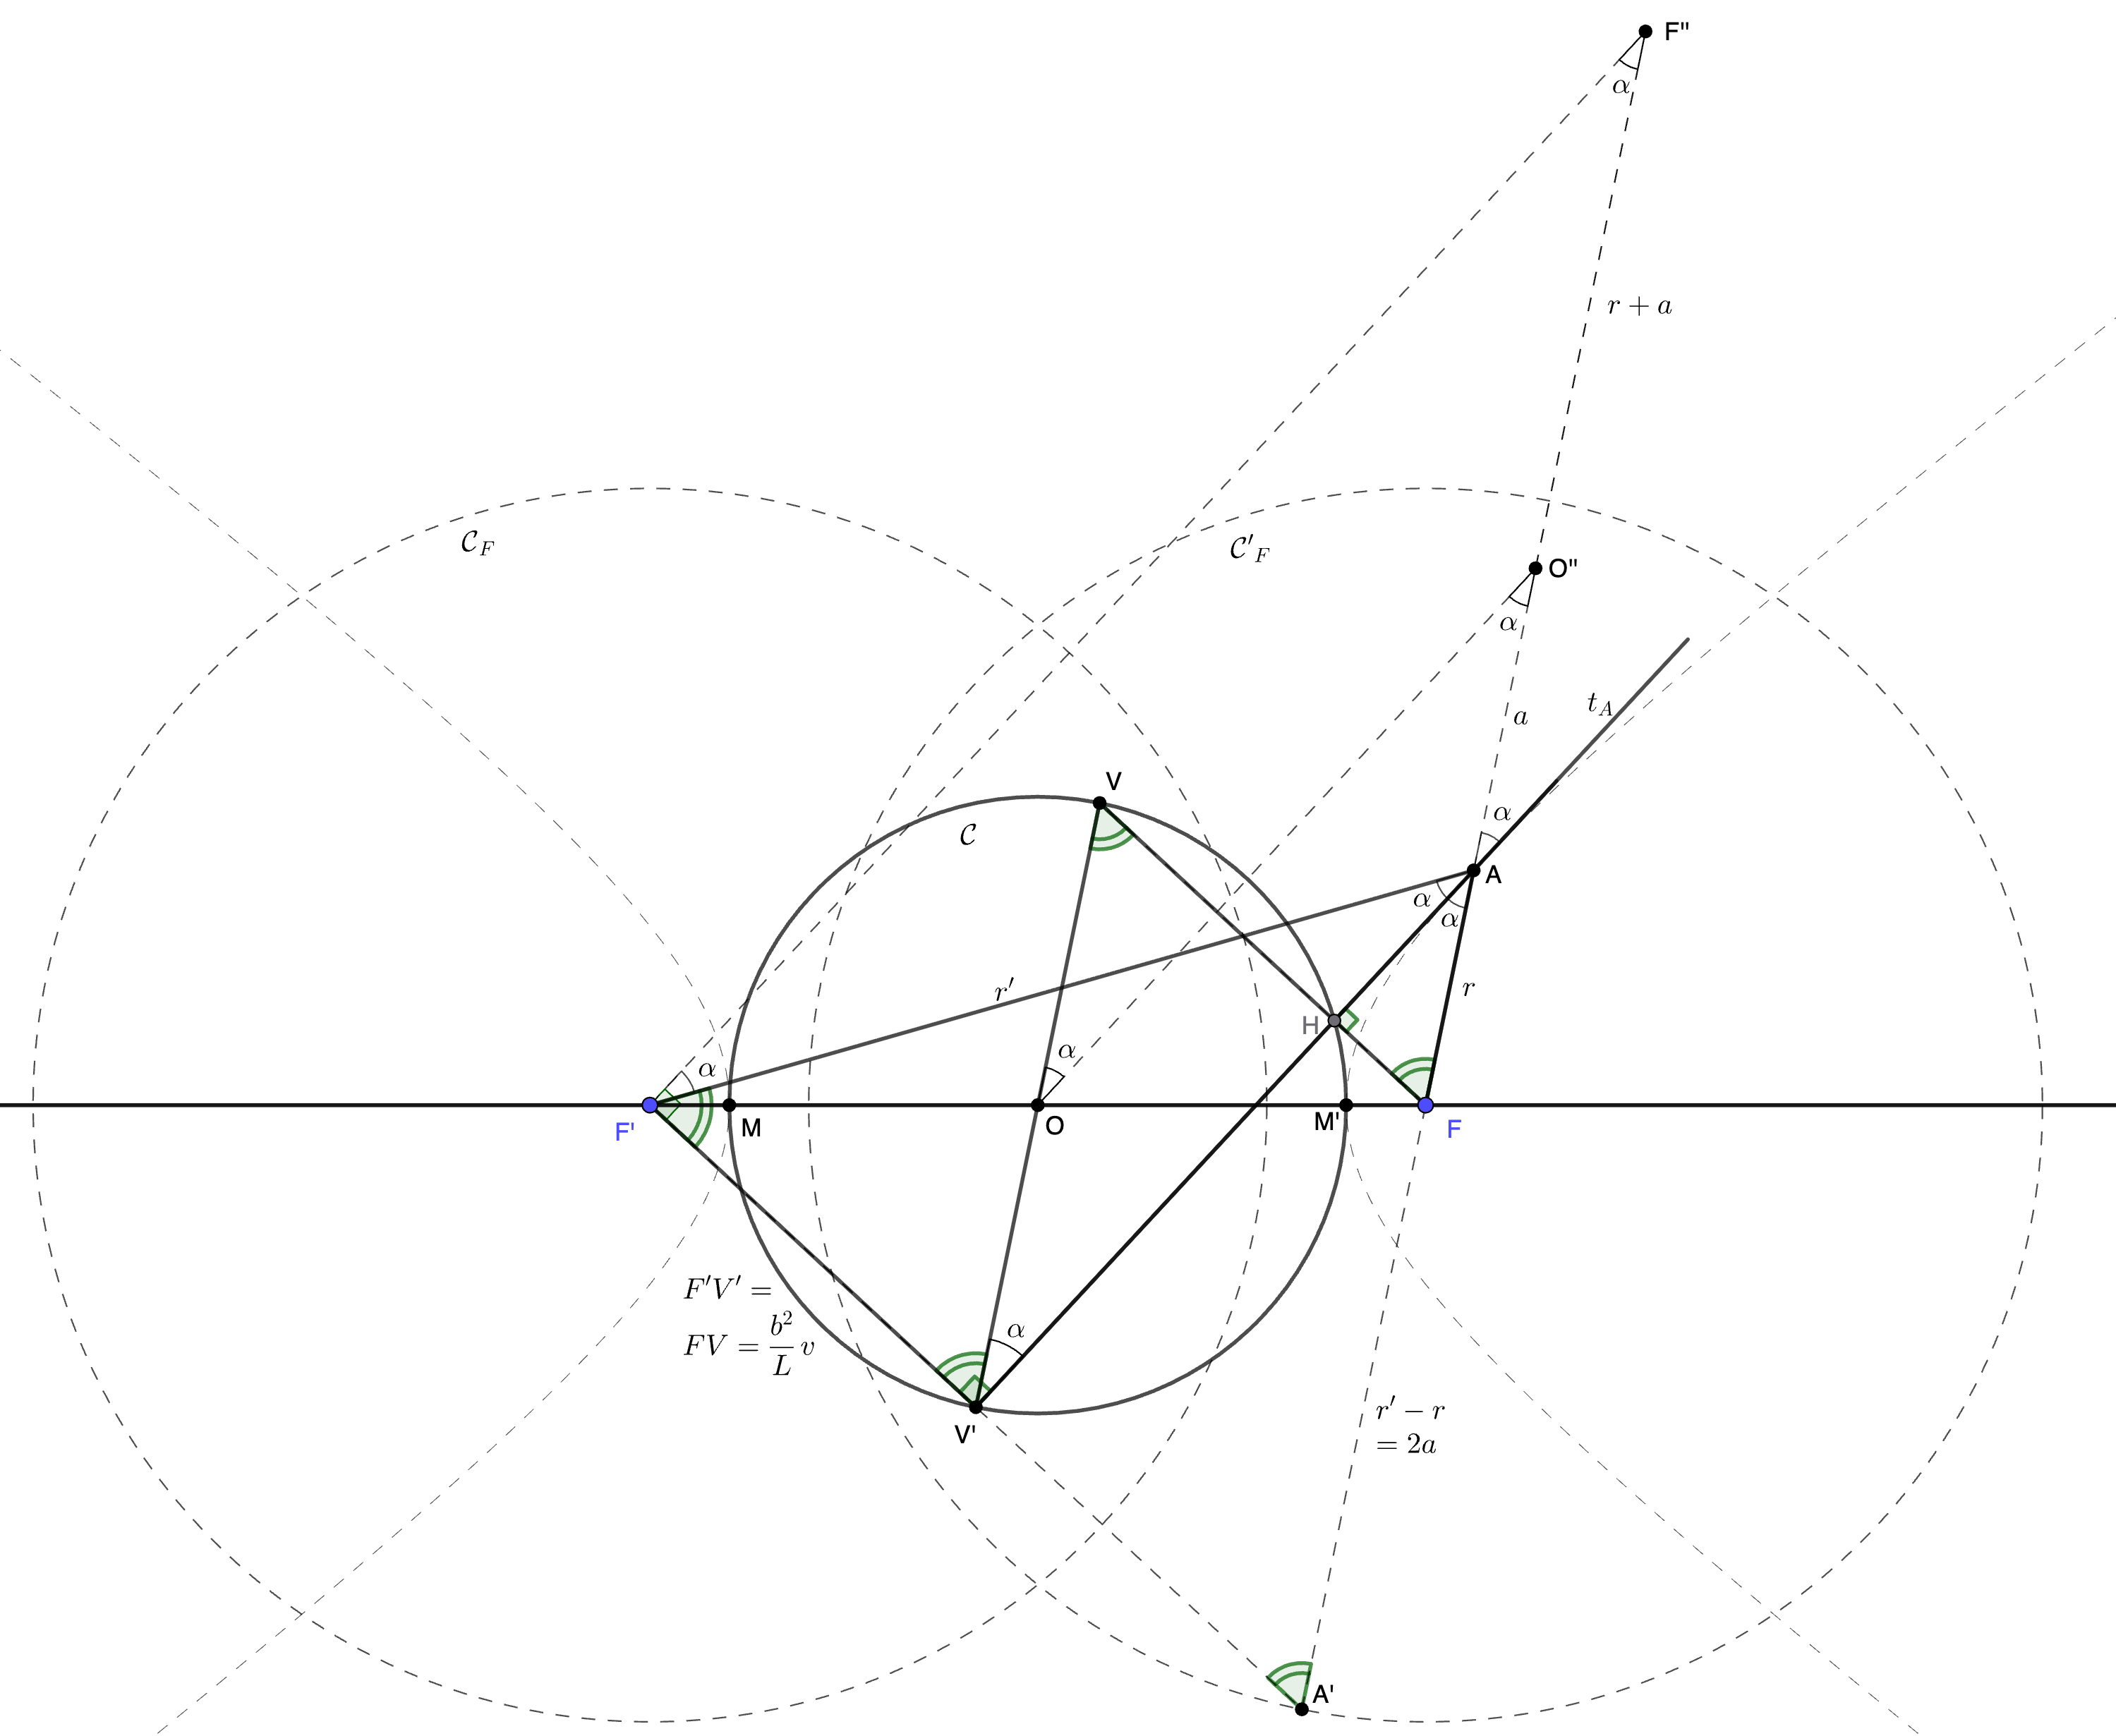
\includegraphics[width=\linewidth]{assets/images/hyperbola_proof2F1.png}
  \caption{Hyperbola configuration for Forward Problem Proof~2F.}
  \label{fig:hyperbola-proof2f}
\end{figure}

Using \Cref{fig:hyperbola-proof2f}, we set up the hyperbolic counterpart with the same hodograph-circle logic and branch-sign adjustments.

\begin{proposition}[Forward Problem Proof~2F: hyperbola case]
Assume inverse-square centripetal attraction, so the hodograph is a circle. If the velocity origin lies outside that hodograph circle, then the orbit is a hyperbola.
\end{proposition}

\begin{proof}
This proof is almost the same as the elliptic proof in \Cref{subsec:ellipse-proof2f}; the same is true for the alternative proof below. The only essential normalization change is
\[
  b^2=c^2-a^2,
\]
which is the hyperbolic identity that matches the rotated/scaled hodograph circle \(\mathcal C\) to the orbit geometry (and the same \(b^2/L\) scale can be rewritten from initial data as in \Cref{subsec:proof2f-discussion}).

With \(OF=c\), \(FV=\frac{b^2}{L}v\), and \(FH=d\), the secant product gives
\[
  FM'\cdot FM=FV\cdot FH=(c-a)(c+a)=c^2-a^2=b^2,
\]
hence \(vd=L\). So the tangent-placement step and the constructions of \(V'\) and \(F'\) proceed exactly as in the ellipse case.

Now set \(r:=AF\) and \(r':=AF'\), and define \(A':=FA\cap F'V'\). The midpoint argument in \(\triangle FF'A'\) is unchanged, yielding
\[
  FA'=2a=V'V.
\]
The reflection property at \(A\) is also unchanged, so \(AA'=AF'=r'\). On the chosen branch (\(A,F,A'\) collinear with \(F\) between \(A\) and \(A'\)),
\[
  r'-r = AA'-AF = FA' = 2a.
\]
This is the gardener characterization of a hyperbola (\(\lvert AF'-AF\rvert=2a\)) with foci \(F,F'\). The remaining line-by-line details are parallel to \Cref{subsec:ellipse-proof2f}.
\end{proof}

\paragraph{Alternative closing step (hyperbola Proof~2F').}
\begin{proof}[Alternative proof (hyperbola 2F')]
The alternative closure from ellipse Proof~2F' transfers directly, with one branch change: construct \(F''\) and \(O''\) on the ray \(FA\) beyond \(A\) (rather than on the segment \(FA\)). Draw \(F'F''\parallel t_A\) and \(OO''\parallel t_A\), meeting the ray \(FA\) at \(F''\) and \(O''\), respectively.

Then \(O''A=OV'=a\), so
\[
  FO''=FA+AO''=r+a.
\]
As before, \(O\) is the midpoint of \(FF'\), and \(OO''\parallel F'F''\), so \(O''\) is the midpoint of \(FF''\). Hence
\[
  FF''=2(r+a),
  \qquad
  AF''=FF''-AF=r+2a.
\]
The same reflection-angle argument gives \(AF''=AF'=r'\). Therefore
\[
  r'=r+2a
  \quad\Longleftrightarrow\quad
  r'-r=2a.
\]
Again, the remaining details are routine parallels of the elliptic case.
\end{proof}

\paragraph{Swapped-focus centrifugal variant.}
\begin{proof}[Swapped-focus centrifugal variant]
The centrifugal-force version follows almost exactly as well. In \Cref{fig:hyperbola-proof2f}, swap the names \(F\leftrightarrow F'\), rename the current \(V'\) as \(H\), and let the line through the new \(F'\) and \(H\) meet \(\mathcal C\) again at the new \(V\). After this relabeling, the rest of the construction and proof chain is sequentially identical, so we omit repetitive details.
\end{proof}

As in \Cref{subsec:ellipse-proof2f}, this subsection keeps the geometry-first derivation; the equivalent initial-data determination of the scaling and conic parameters is deferred to \Cref{subsec:proof2f-discussion}.

\subsection{Parabola: Forward Problem Proof 2F}
\label{subsec:parabola-proof2f}

\begin{figure}[t]
  \centering
  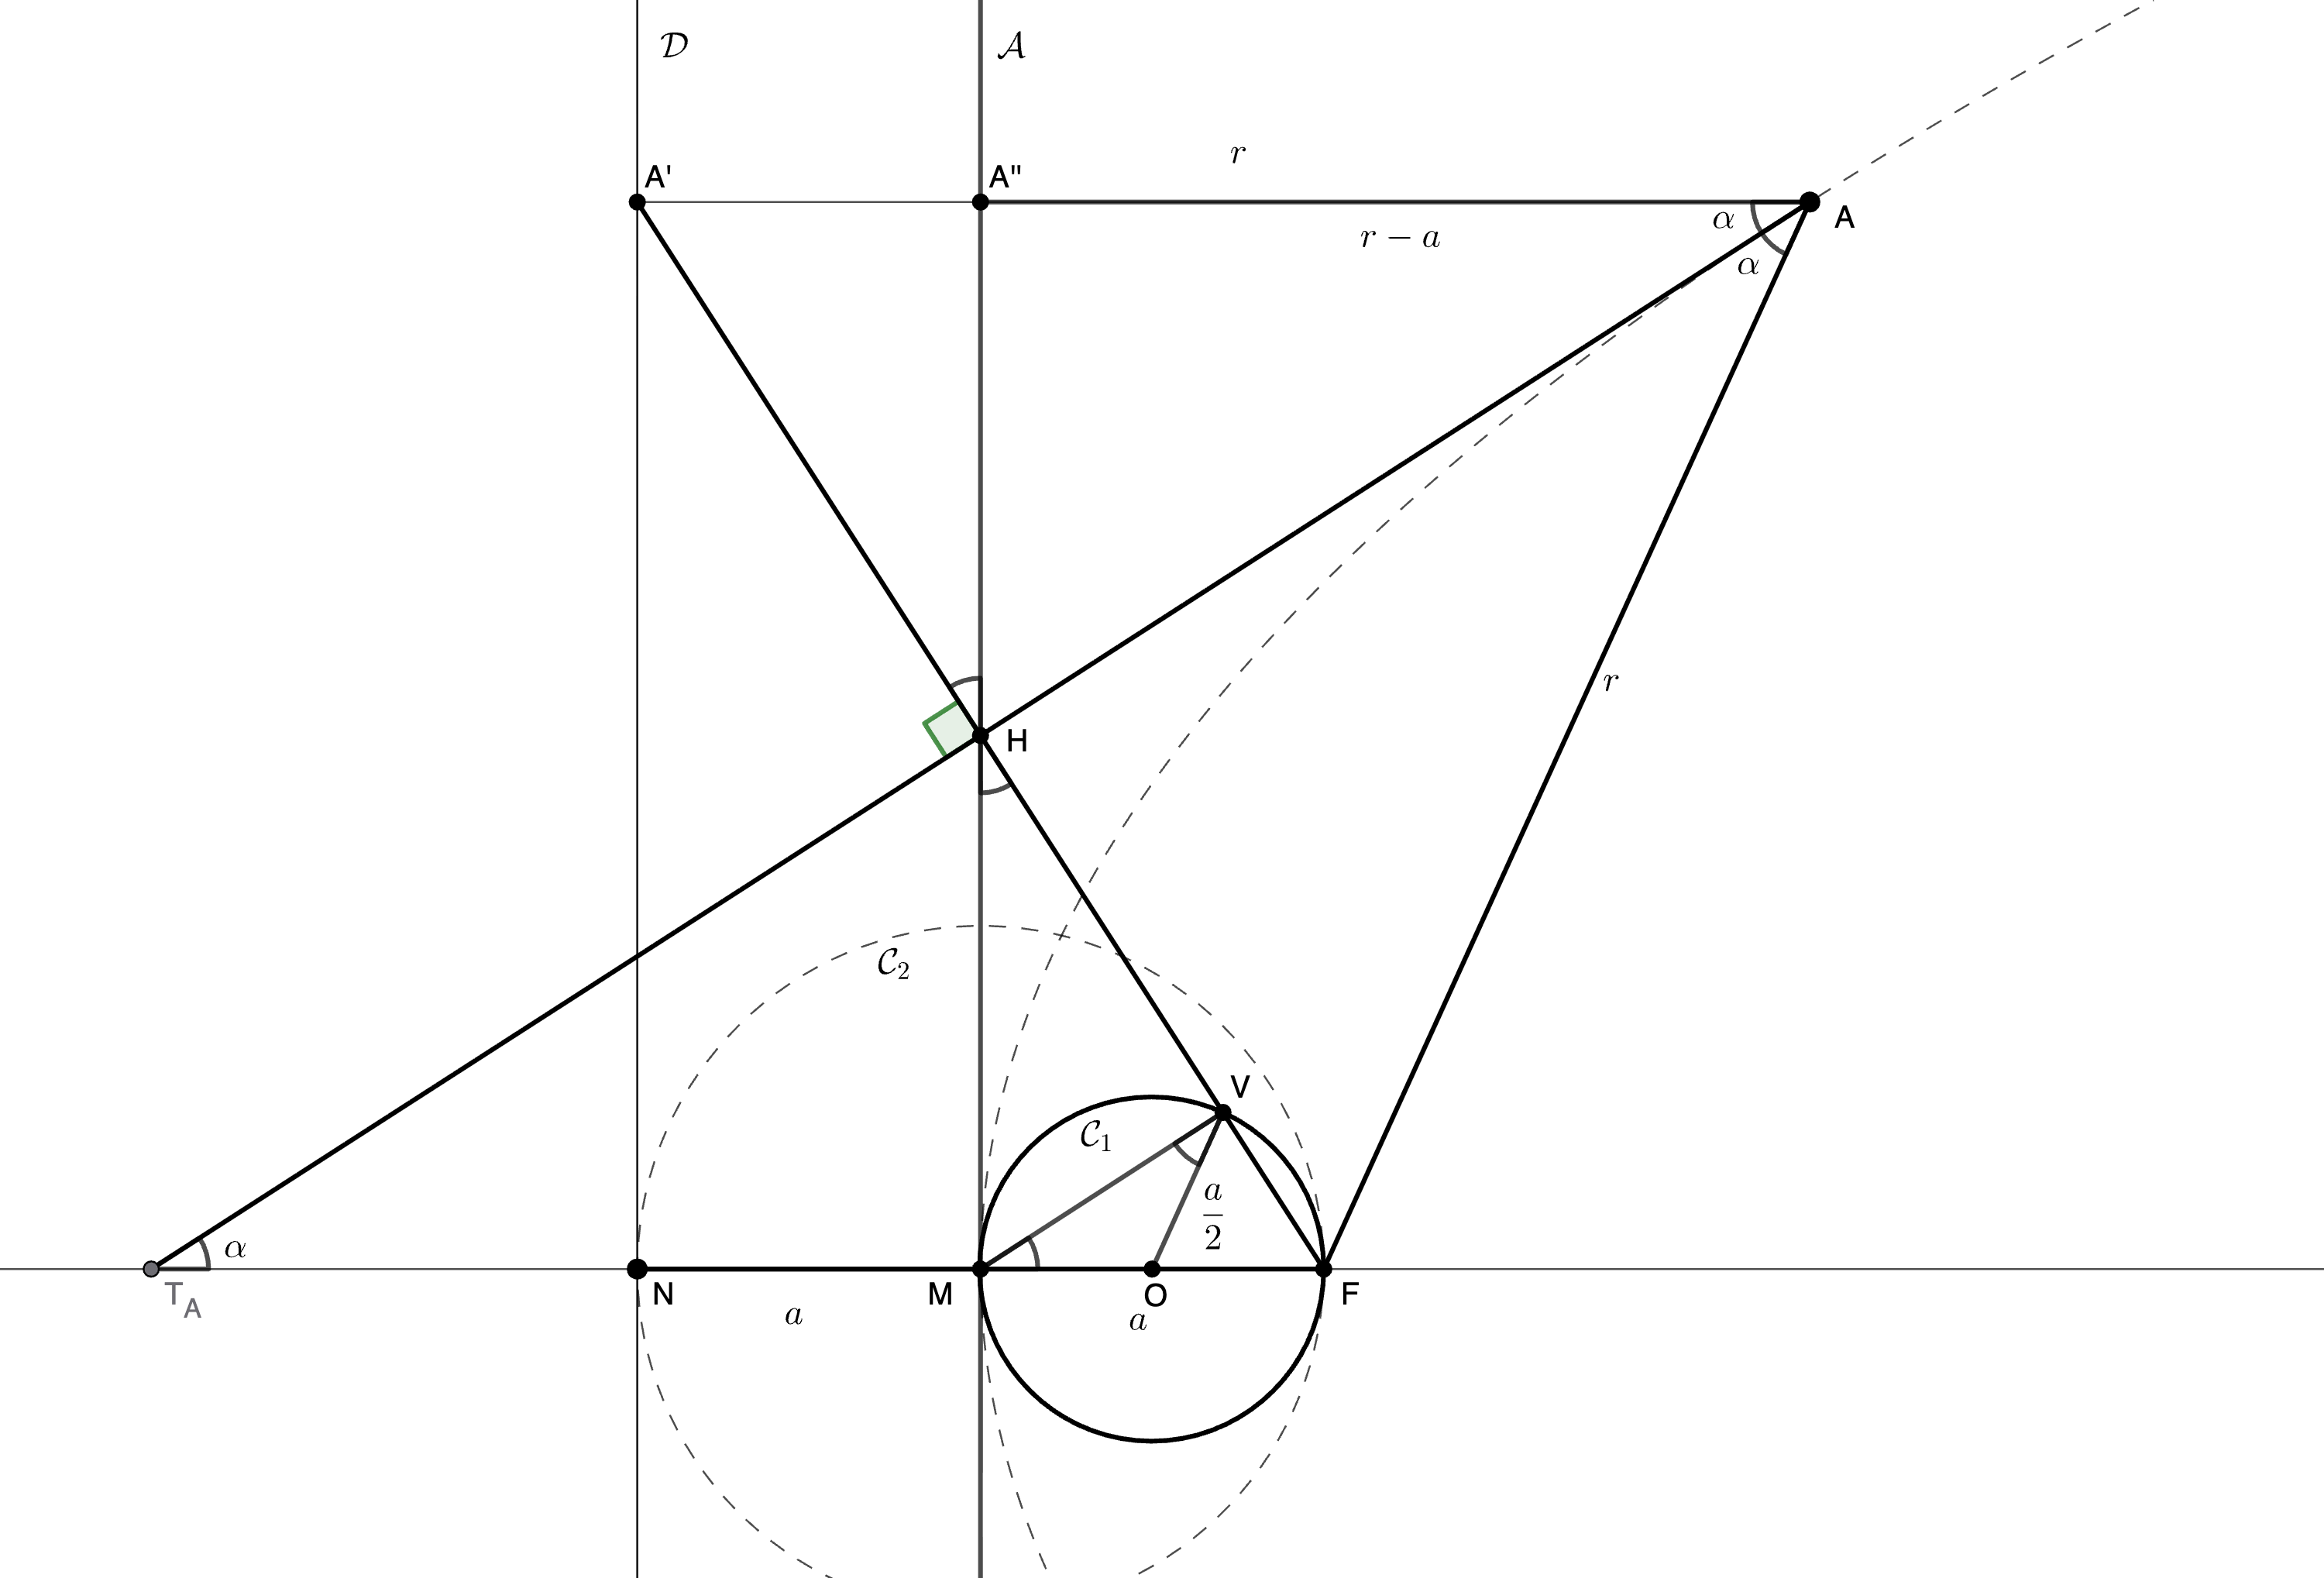
\includegraphics[width=\linewidth]{assets/images/parabola_proof2F.png}
  \caption{Parabola configuration for Forward Problem Proof~2F.}
  \label{fig:parabola-proof2f}
\end{figure}

Using \Cref{fig:parabola-proof2f}, we set up the parabolic threshold case in the same proof family.

\begin{proposition}[Forward Problem Proof~2F: parabola case]
Assume inverse-square centripetal attraction, so the hodograph is a circle. If the velocity origin lies on that hodograph circle, then the orbit is a parabola.
\end{proposition}

\begin{proof}
As in the previous two subsections, rotate the hodograph by \(90^\circ\), but now scale by \(a^2/L\) (with equivalent initial-data form in \Cref{subsec:proof2f-discussion}). In the parabola configuration of \Cref{fig:parabola-proof2f}, the corresponding point \(H\) lies on the fixed line \(\mathcal A\), where \(\mathcal A\perp FM\) and \(FM\) is the diameter of the scaled hodograph circle \(\mathcal C_1\).

For \(V\in\mathcal C_1\), let \(H=VF\cap\mathcal A\). Since \(\triangle MVF\) and \(\triangle HMF\) are right triangles with a common acute angle at \(F\) (because \(V,H,F\) are collinear), they are similar. Hence
\[
  FV\cdot FH=MF^2=a^2.
\]
Using the areal relation \(v\cdot FH=L\), we obtain
\[
  FV=\frac{a^2}{L}\,v,
\]
which is the parabolic analogue of the elliptic/hyperbolic scaling formulas.

Now draw \(t_A\) through \(H\) perpendicular to \(FH\). The orbital point for this \(V\) is
\[
  A:=t_A\cap\{\text{line through }F\text{ parallel to }OV\},
\]
from the same centripetal-direction argument used above.

Let \(T_A:=t_A\cap \overrightarrow{FM}\). Since \(MV\perp VF\) and \(t_A\perp VF\), we have \(MV\parallel AT_A\). Also \(OV\parallel AF\) and \(MO\parallel FT_A\), so \(\triangle A T_A F\sim\triangle VMO\). Therefore the tangent-bisector (reflection) relation is the same as before: the tangent at \(A\) bisects the angle between the focus ray \(AF\) and the fixed direction parallel to \(FM\).

For the directrix closure, draw through \(A\) the line perpendicular to \(\mathcal A\), and let it meet \(\mathcal A\) at \(A''\). By definition \(AF=r\). With the same parallel-line relations,
\[
  AA''=T_A M=F T_A-F M=F A-a=r-a.
\]
Now let \(\mathcal D\parallel\mathcal A\) meet the ray \(FM\) at \(N\) with \(NM=a\). Define \(A'\) as the intersection of ray \(AA''\) with \(\mathcal D\). Then
\[
  AA'=AA''+a=(r-a)+a=r=AF.
\]
Thus the distance to the focus equals the distance to the directrix, which is exactly the defining property of a parabola. (In the plotted construction, \(A',H,F\) are collinear; equivalently, one may define \(A'\) via \(FH\cap\mathcal D\) and verify \(AA'\parallel FM\).) The remaining routine checks are left to the reader.
\end{proof}

\paragraph{Alternative scaled-circle variant.}
\begin{proof}[Alternative scaled-circle variant]
The same conclusion can also be constructed with the auxiliary circle \(\mathcal C_2\) shown in \Cref{fig:parabola-proof2f}, corresponding to a \(2a^2/L\) hodograph scaling (again reducible to initial data as in \Cref{subsec:proof2f-discussion}). As in the ellipse and hyperbola cases, choosing a different but equivalent hodograph proxy changes only intermediate geometric details, not the final parabolic conclusion.
\end{proof}

Again, we postpone the explicit initial-condition parameter map to \Cref{subsec:proof2f-discussion}: this subsection first establishes the geometric mechanism that forces the parabolic form.

\subsection{Discussion}
\label{subsec:proof2f-discussion}

\subsubsection{Initial-Data Parameterization}

Across the ellipse, hyperbola, and parabola cases, Proof~2F and its variants follow one common four-step template. First, rotate and scale the hodograph circle to obtain a geometric proxy in configuration space (with conic-dependent scale choices). Second, combine the secant/product identity with the areal invariant \(L\) so that the tangent carrier \(t_A\) is fixed by the constructed point \(H\). Third, recover the force-center direction by imposing the parallel condition \(AF\parallel OV\), which determines the orbit point on \(t_A\). Fourth, identify the conic through an invariant second focus (ellipse/hyperbola) or invariant directrix (parabola), together with the reflection and gardener/directrix characterization.

This auxiliary-circle framing, imported from the inverse-problem side, gives a concrete pointwise forward construction: each proxy point \(V\) determines a unique orbital point \(A\), rather than relying on a tangent-envelope argument. In this sense, the geometric map from hodograph data to orbit position is explicit at every step.

The same framework also connects cleanly to physical parameters. Equation~(7.1) comes directly from Section~6: \(u=\mu/L\) is the hodograph-circle radius from \Cref{eq:hodo-step3}, and \(p=L^2/\mu\) is the conic polar coefficient from \Cref{eq:proof1f-r-alpha}. Keep only the invariants \(\mu\) and \(L\), then
\begin{equation}
  u=\frac{\mu}{L},
  \qquad
  p=\frac{L^2}{\mu},
\end{equation}
with \(p=\frac{1}{2\kappa}\) from \Cref{eq:kappa-def}.
For ellipse, the equivalent geometric form \(p=b^2/a\) was stated in \Cref{eq:p-b2-over-a-ellipse}.

At an initial orbit point \(A_0\), let
\begin{equation}
  r_0:=FA_0,\qquad d_0:=FH_0,\qquad L=v_0d_0.
\label{eq:proof2f-disc-r0d0L}
\end{equation}
Then
\begin{equation}
  v_{r0}^2=v_0^2-\left(\frac{L}{r_0}\right)^2
  =L^2\!\left(\frac{1}{d_0^2}-\frac{1}{r_0^2}\right).
\label{eq:proof2f-disc-vr0}
\end{equation}
From \Cref{eq:proof1f-r-alpha}, \(r=p/(1-e\cos\alpha)\), so at \(A_0\),
\begin{equation}
  e\cos\alpha_0=1-\frac{p}{r_0},
  \qquad
  e\sin\alpha_0=\frac{p}{L}v_{r0},
\label{eq:proof2f-disc-e-alpha0}
\end{equation}
hence
\begin{equation}
  e^2
  =\left(1-\frac{p}{r_0}\right)^2+\frac{p^2}{L^2}v_{r0}^2
  =1+\frac{p^2}{d_0^2}-\frac{2p}{r_0}.
\label{eq:proof2f-disc-e2-initial}
\end{equation}
Define
\begin{equation}
  E_0:=\frac{v_0^2}{2}-\frac{\mu}{r_0}
  =\frac{L^2}{2d_0^2}-\frac{\mu}{r_0},
\label{eq:proof2f-disc-E0}
\end{equation}
where \(L=v_0d_0\).
Then
\begin{equation}
  e^2=1+\frac{2E_0L^2}{\mu^2},
\label{eq:proof2f-disc-e2-E0}
\end{equation}
so the regime is
\begin{equation}
  E_0<0\ (\text{ellipse}),\qquad
  E_0=0\ (\text{parabola}),\qquad
  E_0>0\ (\text{hyperbola}),
\end{equation}
consistent with \Cref{eq:proof1f-regimes}.

For ellipse/hyperbola, \(e=c/a\), \(p=b^2/a\), and \(s_{\mathrm{hodo}}=b^2/L\). For parabola (with \(a:=MF\) in \Cref{subsec:parabola-proof2f}), \(p=2a\) and \(s_{\mathrm{hodo}}=a^2/L\). Using \(2E_0=v_0^2-\frac{2\mu}{r_0}\), the initial-data form simplifies to
\begin{equation}
  s_{\mathrm{hodo}}
  =
  \begin{cases}
    -\dfrac{L}{2E_0}, & E_0<0,\\[8pt]
    \dfrac{L^3}{4\mu^2}, & E_0=0,\\[8pt]
    \dfrac{L}{2E_0}, & E_0>0.
  \end{cases}
\label{eq:proof2f-disc-shodo-E0}
\end{equation}
Using \(u=\mu/L\), this gives
\begin{equation}
  a=s_{\mathrm{hodo}}\,u
  =
  \begin{cases}
    -\dfrac{\mu}{2E_0}, & E_0<0,\\[8pt]
    \dfrac{L^2}{4\mu}, & E_0=0,\\[8pt]
    \dfrac{\mu}{2E_0}, & E_0>0.
  \end{cases}
\label{eq:proof2f-disc-shodo-u-E0}
\end{equation}
For non-parabolic conics \((E_0\neq 0)\), this is equivalent to
\begin{equation}
  a=\frac{\mu}{2|E_0|},
  \qquad
  b^2=ap=\frac{L^2}{2|E_0|},
  \qquad
  c=ae,\quad
  e=\sqrt{1+\frac{2E_0L^2}{\mu^2}},
\label{eq:proof2f-disc-abc-from-initial}
\end{equation}
so \(a,b,c\) are all fixed by initial data \((\mu,L,r_0,d_0)\).
Equation~\eqref{eq:proof2f-disc-shodo-u-E0} is equivalently the hodograph-scaling statement emphasized in van Haandel--Heckman and then used directly in the CRS treatment \cite{vanhaandelheckman2009teaching,carinena2016newlook}.
So the geometric scaling in Proof~2F is fixed directly by initial dynamical data.

\subsubsection{Orbit-Wide Form and Conserved Specific Energy}

The derivation above is not tied to the special notation \(r_0,v_0,d_0\). Equations~\eqref{eq:proof2f-disc-vr0}--\eqref{eq:proof2f-disc-e2-E0} apply at any point \(A\) on the same orbit by replacing
\[
  (r_0,v_0,d_0,E_0)\ \mapsto\ (r,v,d,E),
\]
with
\[
  L=vd,\qquad E:=\frac{v^2}{2}-\frac{\mu}{r}.
\]
Then the same algebra gives
\begin{equation}
  e^2=1+\frac{2EL^2}{\mu^2}.
\label{eq:proof2f-disc-e2-E}
\end{equation}
Since \(\mu\) is fixed by the force law, \(L\) is fixed by central-force areal invariance, and \(e\) is the global eccentricity of one conic orbit, \Cref{eq:proof2f-disc-e2-E} implies that \(E\) is constant along the orbit. Thus this geometric framework also recovers conservation of specific mechanical energy. Multiplying by the planet mass gives the usual total-energy conservation statement.

This does not claim energy conservation must be derived from \Cref{eq:proof1f-regimes} or from one specific geometric route; conservation of energy is broader. But within the forward-problem discussion, it is useful to state explicitly that the same geometric invariants imply it. Many forward-problem expositions take energy as a starting law (or derive it by integration first, then use geometry), as in the pedagogical lines discussed by Markowsky, van Haandel--Heckman, and Simha \cite{markowsky2011newton,vanhaandelheckman2009teaching,simha2021algebra}.

\subsubsection{Kepler's Third Law and Universal Gravitation}

For the elliptic case, Section~3 gives the area by affine-circle mapping:
\[
  \mathrm{Area}(\text{orbit})=\pi ab.
\]
Since \(L\) is twice areal speed, one full period satisfies
\begin{equation}
  T=\frac{\pi ab}{L/2}=\frac{2\pi ab}{L}.
\label{eq:proof2f-disc-period}
\end{equation}
Using \(b^2=ap\) and \(p=L^2/\mu\),
\begin{equation}
  T^2
  =\frac{4\pi^2a^2b^2}{L^2}
  =\frac{4\pi^2a^3p}{L^2}
  =\frac{4\pi^2}{\mu}\,a^3,
\label{eq:proof2f-disc-third-law}
\end{equation}
hence
\begin{equation}
  \frac{T^2}{a^3}=\frac{4\pi^2}{\mu}=\text{constant}
\label{eq:proof2f-disc-third-law-ratio}
\end{equation}
for all bodies orbiting the same center (same \(\mu\)).

This is the Kepler-third-law form in the present notation. Combined with \( \mathbf F=m\,\mathbf a\), it leads to the inverse-square force model
\[
  \mathbf a=-\frac{\mu}{r^2}\,\hat{\mathbf r},
  \qquad
  \mathbf F=-\frac{\mu\,m_{\mathrm p}}{r^2}\,\hat{\mathbf r}.
\]
By two-body symmetry, \(\mu\) is proportional to the source mass; for solar orbits, \(\mu=G M_\odot\), giving
\[
  \mathbf F=-\frac{G M_\odot m_{\mathrm p}}{r^2}\,\hat{\mathbf r}.
\]
The mass-independence of \(\mathbf a\) in this form is precisely the empirical content of the proportionality between inertial and gravitational mass. Newton's comparison of lunar orbital acceleration with near-Earth free fall is the classical argument for universality. For historical and modern accounts, see the \emph{Principia} sources and reconstructions \cite{newton1687principia,newton1846mottewikisource,newton1934mottecajori,chandrasekhar1995principia,nauenberg2003keplerarea,markowsky2011newton}.

Historically, the route from the third law to gravitation also required a nontrivial geometric step: to place terrestrial gravity and lunar motion under one law, Newton had to control the effects of extended bodies. In the \emph{Principia} he proved the spherical-symmetry (shell) result---an external body is attracted by a spherically symmetric mass as if all its mass were concentrated at the center---thereby making the inverse-square model physically applicable to planets and stars. Coupled with the Moon-versus-surface-fall comparison, this supports the universality claim. The same work also gives geometric treatments of barycentric motion (e.g., Sun--Jupiter), curvature--force relations, and time-of-flight constructions, illustrating how Newton extended Euclidean geometry into dynamics by introducing time into spatial constructions; modern analytical mechanics rewrites much of this in calculus form, but the underlying geometric architecture remains rich and continues to generate interest for deeper dives \cite{newton1687principia,newton1846mottewikisource,newton1934mottecajori,chandrasekhar1995principia,markowsky2011newton}.

To close the forward-problem arc: once the initial data are given, \Cref{eq:proof2f-disc-r0d0L,eq:proof2f-disc-shodo-E0,eq:proof2f-disc-shodo-u-E0,eq:proof2f-disc-abc-from-initial} uniquely fix the rotated/scaled hodograph proxy (its size and orientation) and the corresponding force-center placement in that proxy geometry. From there, the remaining construction follows exactly the same flow as \Cref{subsec:ellipse-proof2f,subsec:hyperbola-proof2f,subsec:parabola-proof2f}. This is why we chose the present order: first show geometrically why conic structure is inevitable, then use initial conditions only to select the exact member (shape and scale) within that conic family.
